\documentclass[conference]{IEEEtran}
\usepackage{graphicx,cite,bm,psfrag,amsmath}
\def\mmax{\mathop{\mbox{\scriptsize max}}}
\def\argmin{\mathop{\mbox{arg\,min}}}
\def\argmax{\mathop{\mbox{arg\,max}}}
\newcommand{\defequal}{\stackrel{\mathrm{def}}{=}}
\renewcommand{\vec}[1]{{\ensuremath{\boldsymbol{#1}}}}
\newcommand{\popt}{\ensuremath{P^{(K)}_{opt}}}
\IEEEoverridecommandlockouts
\pagestyle{plain}
\usepackage{amsfonts}
\usepackage{algorithm, algorithmic}
\renewcommand{\algorithmicrequire}{ \textbf{Input:}} %Use Input in the format of Algorithm
\renewcommand{\algorithmicensure}{ \textbf{Procedures:}} %UseOutput in the format of Algorithm
% correct bad hyphenation here
%\hyphenation{op-tical net-works semi-conduc-tor}
\usepackage{CJK}
\usepackage{color}
\usepackage{url}
\usepackage{geometry}
\geometry{left=0.5in, right=0.5in, top=0.75in, bottom=0.75in}

\begin{document}
\title{Group Clustering for Block Diagonal Digital Precoder in Multi-user MIMO System}
\author{\IEEEauthorblockN{Guanchong Niu, Qi Cao and Man-On Pun\IEEEauthorrefmark{3}
%\IEEEauthorrefmark{3},
\IEEEauthorblockA{
School of Science and Engineering\\
The Chinese University of Hong Kong, Shenzhen\\
Shenzhen, Guangdong, China, 518172
%\thanks{This work was supported, in part, by the CUHKSZ President's Fund under Grant No. PF.01.000211 and  Shenzhen Science and Technology Innovation Committee under Grant No. ZDSYS20170725140921348.} \thanks{\IEEEauthorrefmark{3} Corresponding author, email: SimonPun@cuhk.edu.cn.}
}}}


\maketitle \thispagestyle{plain}
\pagenumbering{gobble}
\begin{abstract}
Beam division multiple access (BDMA) has recently been proposed for massive multiple-input multiple-output (MIMO) systems by simultaneously transmitting multiple users' data streams via different beams. Meanwhile, the block hybrid precoding has been proposed to reduce the computational complexity. However, previous works mostly rely on a crucial condition that the number of RF chains must be not less than the number of data streams. In this paper, we propose a multipath BDMA based hybrid block precoding system to break the ceiling on minimal required RF chains where the data streams are processed cluster-by-cluster. To overcome the performance degradation arisen from block hybrid precoding scheme, a K-means based heuristic user clustering algorithm is proposed to minimize the inter-cluster interference. Then two digital precoding approaches are investigated to suppress the intra-cluster interference by separately considering the signal-to-interference-and-noise ratio (SINR) and signal-to-leakage-and-noise ratio (SLNR).   Simulation results confirm the effectiveness of proposed block clustering precoding scheme compared to conventional hybrid beamforming scheme.
\end{abstract}

\section{introduction}
To meet the ever-increasing demand of higher user data rates, it is envisioned that the next-generation cellular systems will be equipped with massive antenna arrays \cite{boccardi2014five}. Capitalizing on the large number of antennas at the base-station (BS), beam division multiple access (BDMA) has recently been proposed to transmit multiple users' data-streams via different beams \cite{sun2015beam, Jiang2018}. In contrast to the more conventional multiple access schemes such as Code Division Multiple Access (CDMA) or Orthogonal Frequency Multiple Division Access (OFDMA) that multiplex users in code, time and frequency domains, BDMA separates users in the beam space by transmitting data to different users in orthogonal beam directions. In \cite{sun2015beam}, BDMA was first proposed to decompose the multiuser multiple-input multiple-output (MU-MIMO) system into multiple single-user MIMO channels by multiplexing multiple users' data onto non-overlapping beams. More recently, joint user scheduling and beam selection for BDMA was formulated under the Lyapunov-drift optimization framework before the optimal user-beam scheduling policy was derived in a closed form \cite{Jiang2018}. However, the assumption of non-overlapping orthogonal beams is hard to be satisfied which limits the potential of analog-only BDMA beamforming solution. Different from analog-only beamforming system, digital precoding can be implemented to eliminate the inter-user interference, where the baseband requires dedicated RF chain per each antenna\cite{bogale2014beamforming}.

However, the expensive and power-hungry components (e.g. ADC/DAC, filters, mixers and amplifiers) in RF chain constitute an impediment of broad implementation of massive MIMO systems.  Thus, hybrid digital and analog beamforming has been developed for massive MIMO transmissions by dividing the procoding process into two steps, namely analog and digital precoding \cite{han2015large, el2014spatially}. More specifically, the transmitted signals are first precoded digitally using a smaller number of radio frequency (RF) chains followed by the analog precoding implemented with a much larger number of low-cost phase shifters. As a result, the hybrid analog-digital precoding architecture requires significantly less RF chains as compared to the fully digital precoding in which every available antenna element is supported by one RF chain. 

To further reduce the computational complexity and obtaining closed-form solutions in downlink space-division multiple access (SDMA), the notion of \textit{block diagonalization} (BD) was introduced in \cite{spencer2004zero}, which is found out helpful in massive MIMO transmissions especially for digital precoder design of hybrid beamforming system. This is because computation and implementation of full zero-forcing precoding matrix in an instant is of great challenge, while separating digital precoders into blocks efficiently mitigates the hard work. With the number of transmit RF chains larger than the total number of receive RF chains (considering multiuser scenario), it can be achieved that, for each block, base station projects all inter-block interference onto the its null spaces \cite{ni2016hybrid}. By setting up an optimization problem minimizing the means square error (MSE) between the received signals resulted from full ZF prcoding system and BD precoding system, \cite{bogale2014beamforming} indicates that utilizing BD precoders can realize an asymptotic performance to full ZF precoding transmissions. Actually, the composition of a block is flexible, \textit{i.e.} it can be a downlink user with multiple antennas or multiple single-antenna users. For instance, in \cite{liu2014phase}, the structure of hybrid BD precoding is also investigated but with each block being a group of single-antenna users. In such a system, the size of each block can even be a optimization variable. Nevertheless, the above hybrid BD massive MIMO systems are all under a crucial condition, that is, the number of RF chains must be no less than the number of supported data-streams.

To circumvent the restriction, \cite{garcia2017mimo} uses $L$ RF chains to approximate $K\geq L$ transmitted symbols, in this way, the data-stream to RF chain ratio can be above 1. The success of this scheme relies on that the state-of-art phase shifters and switches can change their state in hundreds of pico seconds, since the approximation needs to be done in each symbol period. However, due to that digital/analog precoder is symbol-dependent, and users have to recover symbols via compressive sensing tools, the overall scheme is of high complexity. In this paper, we also consider the hybrid BD multiuser massive MIMO system with number of data-streams larger than number of RF chains, and against the current literature, our contributions are threefold:

\begin{figure*}[t]
\centering
\begin{minipage}[t]{0.7\linewidth}
	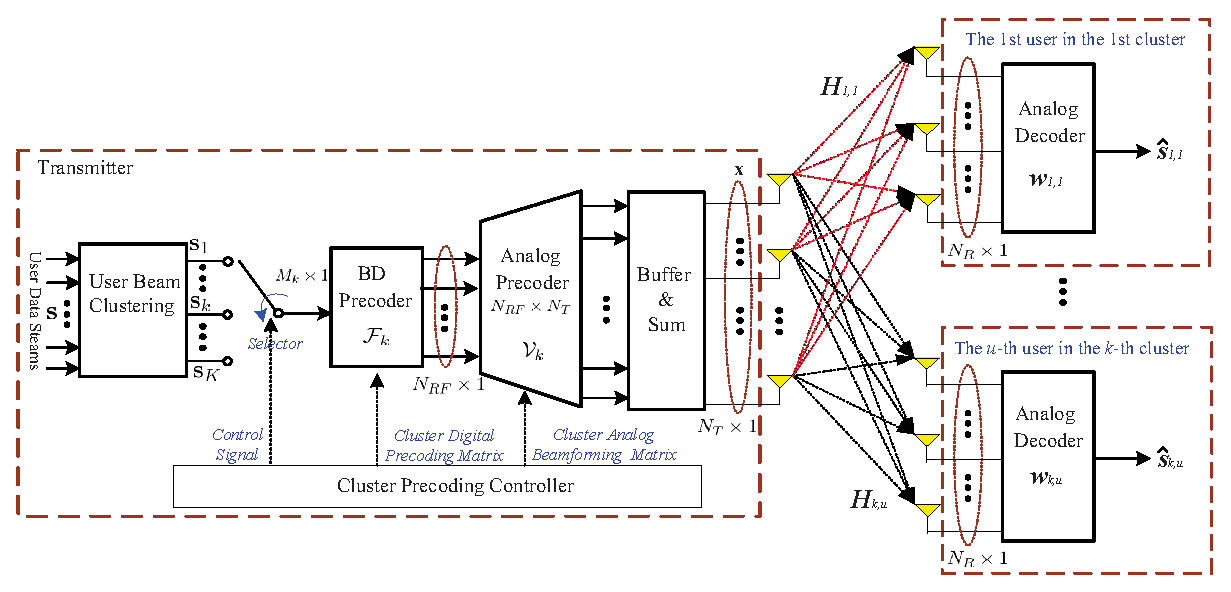
\includegraphics[width=5.6in,height=3in]{PPTFigure/BlockDiagonal.eps}
	\caption{Block diagram of the hybrid precoding system under consideration}\label{fig:BlockDiagram}
	\parbox{6.5cm}{\small \hspace{1.5cm} }
\end{minipage}
\end{figure*}

\begin{itemize}
\item It is widely accepted in massive MIMO studies that the number of data-streams is restricted to the number of RF chains. To break the rule, we propose a cluster-by-cluster hybrid precoding process that involves both digital and analog precoders. In our proposed scheme, users are divided into $K$ clusters, their signals are multiplied by corresponding digital precoders block by block, and added up together at the analog precoding stage before simultaneous transmission. Thus, the data-stream per physical RF chain is far above 1 while the data-stream per RF chain usage is still equal to 1.
\item Clustering different users together results in different systematic performance. This phenomenon is also known as peer effect. For particular digital and analog precoding strategy, we formulate the user clustering problem as an integer programming problem, which is of NP-hardness. To tackle the problem, we propose a K-means based heuristic user clustering greedy algorithm that could effectively improve system sume-rate capacity.
\item We design a whole set of transmission scheme from transmit digital/analog precoding matrix to the receive analog beamforming vectors. With finite number of transmit antennas, the inter-cluster interference inherently exists in our system model, hence we investigate two distinguishing digital precoders respectively coming from equivalent channel inversion and signal-to-leakage-and-noise (SLNR), which show equivalent performance in simulation results.
\end{itemize}



The structure of this paper is arranged as follows: the massive MIMO system with asynchronous hybrid BD precoding is introduced in Section II; the design of transmit digital/analog precoding matrix and receive analog beamforming vectors are elaborated in Section III; The user clustering algorithm is detailed in Section IV whereas the simulation results are shown in Section V; and finally we conclude the paper in Section VI

\underline{Notation}: Vectors and matrices are denoted by boldface letters. $\bm{I}_N$ denotes the identity matrix with size $N\times N$. ${\bm A}^T$ and ${\bm A}^H$ denote transpose and conjugate transpose of ${\bm A}$, respectively. $\bm{A}^\dagger$ being the pseudo inverse of $\bm{A}$ while $||\bm{A}||_0$, $||\bm{A}|| $ and $|\bm{A}|$ stand for $0$ norm, the Frobenius norm and determinant of ${\bm A}$, respectively. $\bm{A}(i,j)$ denotes the $i$ row, $j$ column element of ${\bm A}$; $|\mathcal{I}|$ is the cardinality of the enclosed set ${\cal I}$; Finally, $\mathbb{E}[\cdot] $ and $\Re\{\cdot\}$ denote the expectation and real part of a random variable.

\section{system model}
There are $N_{tot}$ users under considered base station, and $N_U$ of them will be selected to serve. We consider a multi-user mmWave MIMO system shown in \figurename{ \ref{fig:BlockDiagram}}, in which a transmitter equipped with $N_{RF}$ RF chains and $N_T$ antennas transmits $N_U$ data streams to $N_U$ receivers with $N_R$ receive antennas. Following the same assumption commonly employed in the literature \cite{alkhateeb2015limited}, we assume only one data stream is designated to each scheduled receiver. We use ${\bm s}(n)$ to denote the $n$-th block of $N_U$ data to be transmitted with $\mathbb{E}\left[\bm{ss}^H\right]=\frac{1}{N_U}\bm{I}_{N_U}$. In the sequel, we concentrate on a single block and omit the temporal index $n$ for notational simplicity.

Many papers have proposed block algorithm to reduce the computational complexity. Our basic idea is to group the users into several clusters and then the inter-cluster interference can be minimized by analog precoding with group-scheduling and the intra-cluster interference can be eliminated by digital precoding.

The $N_U$ users are divided into $K$ clusters and each cluster has $M_k$ users. Obviously, we have
\begin{equation}
	\sum_{k=1}^{K} M_k = N_U, \quad 0< M_k\leq N_U
\end{equation}

And the digital precoder is given by 
\begin{equation}
\bm{F} = 
\begin{bmatrix}
\bm{\mathcal{F}}_1&\cdots & \bm{0}&\bm{0}\\
\vdots & \bm{\mathcal{F}}_2 & \vdots&\vdots \\
\bm{0}&\cdots&\ddots &\bm{0}\\
\bm{0}&\cdots & \bm{0}&\bm{\mathcal{F}}_K
\end{bmatrix}
,\quad
\bm{F}_k \in \mathcal{C}^{N_{RF}\times M_k}
\end{equation}

Correspondingly, the analog precoder is also divided into $K$ parts
\begin{equation}
	\bm{V} = \left[\bm{\mathcal{V}}_1, \bm{\mathcal{V}}_2,\cdots, \bm{\mathcal{V}}_{K}\right], \quad \bm{\mathcal{V}}_k\in \mathcal{C}^{N_T\times M_k}
\end{equation}
Also, the data streams $\bm{S}$ is divided into $K$ clusters
\begin{equation}
\bm{s} = \left[{\mathbf{s}}_1^T, {\mathbf{s}}_2^T,\cdots, \mathbf{s}_{K}^T\right]^T, \quad \mathbf{s}_k\in \mathcal{C}^{M_j\times 1}
\end{equation}

For conventional block hybrid precoding systems, the number of required RF chains is still equal to the number of users although the computational complexity is reduced. Distinct to the conventional systems, each RF chain can serve more than one data stream thus the required RF chains will be significantly reduced in our proposed cluster-by-cluster hybrid precoding system as shown in Fig. \ref{fig:BlockDiagram}.

We use $\bm{f}_{ku}, \bm{v}_{ku}$ and $s_{ku}$ to represent the digital precoding, analog precoding and data stream for $u$-th user in $k$-th cluster.

The resulting precoded signal $\bm x$ of dimension $N_T\times 1$  can be expressed as
\begin{equation}{\label{eq:transx}}
{\bm x} =  \bm{V}\cdot \bm{F}\cdot\bm{s} =\sum_{k=1}^K \bm{\mathcal{V}}_k \bm{\mathcal{F}}_k \mathbf{s}_k
\end{equation}

The precoded signal $\bm x$ is then broadcast to $N_U$ users. The signal received by the $u$-th user is given by

\begin{eqnarray}{\label{eq:rewrite}}
{\bm y}_{ku} &=&\underbrace{\bm{H}_{ku} \bm{\mathcal{V}}_k\bm{f}_{ku}{s}_{ku}}_\text{Desired Signal}+\underbrace{\bm{H}_{ku} \bm{\mathcal{V}}_k\sum_{\substack{i=1 \\ i\neq u}}^{M_K}\bm{f}_{ki}s_{ki}}_\text{Intra-cluster Interference} \nonumber\\
&+& \underbrace{\bm{H}_{ku}\sum_{\substack{j=1\\j\neq k}}^{K}\bm{\mathcal{V}}_j\bm{\mathcal{F}}_j\bm{s}_j}_\text{Inter-cluster Interference}+ \underbrace{\bm{n}_{ku}}_\text{Noise}
\end{eqnarray}
where $\bm{H}_{ku}$$\in\mathbb{C}^{N_R\times N_T}$ is the MIMO channel matrix between the transmitter and the $u$-th receiver\cite{el2014spatially}. Furthermore, $\bm{n}_u$ is complex additive white Gaussian noise with zero mean and variance equal to $\sigma^2$.

Assuming the receivers are all low-cost terminals that perform analog beamforming only in decoding, the decoded signal by the $u$-th user in $k$-th cluster denoted by $\hat{s}_u$ is given as
\begin{equation}{\label{eq:hats}}
\hat{s}_{ku} = \bm{w}_{ku}^H \bm{H}_{ku} \bm{\mathcal{V}}_k \bm{f}_{ku} s_{ku} + \bm{w}_{ku}^H \bm{\tilde{n}}_{ku},
\end{equation}
where ${\bm w}_{ku}$ of dimension $N_R\times 1$ is the analog beamforming vector employed by the $u$-th receiver with the power constraint of $|\bm{w}_u|^2=1$ and
\begin{equation}\label{Eq:ntilde}
\bm{\tilde{n}}_u=\bm{H}_{ku} \bm{\mathcal{V}}_k\sum_{\substack{i=1 \\ i\neq u}}^{M_K}\bm{f}_{ki}s_{ki} + \bm{H}_{ku}\sum_{\substack{j=1\\j\neq k}}^{K}\bm{\mathcal{V}}_j\bm{\mathcal{F}}_j\bm{s}_j+  \underbrace{\bm{w}_{ku}^H \bm{n}_{ku}}_\text{Noise}
\end{equation}
Note that the first term in Eq.~(\ref{eq:hats}) stands for the desired signal while the second term is the sum of its own receiver noise and interference from intra-cluster users and other clusters' users.

\subsection{Channel Model}
As shown in \cite{rappaport2014millimeter}, the mmWave wireless channel can be well modeled by the Saleh-Valenzuela model. Following the same approach developed in \cite{alkhateeb2014channel}, we assume that each scatter only contributes one single propagation path. As a result, the $u$-th user's channel model can been modeled as:
\begin{equation}{\label{eq:Hu}}
\bm{H}_u = \sqrt{\frac{N_{T}N_{R}}{L_{u}}}\sum_{l=1}^{L_u}\alpha_{u,l}\cdot \bm{a}_{R}(\phi^r_{u,l},\theta^r_{u,l}) \cdot\bm{a}_{T}^{H}(\phi^t_{u,l},\theta^t_{u,l}),
\end{equation}
where $L_u$ is the number of scatters of the $u$-th user's channel. Furthermore, $\alpha_{u,l}$, $\theta^r_{u,l}/\phi^r_{u,l}$ and $\theta^t_{u,l}/\phi^t_{u,l}$ are the complex path gain, azimuth/elevation angles of arrival(AoA) and azimuth/elevation angles of departure(AoD) of the $l$-th path of the $u$-th user, respectively. Finally, ${\bm a}$ is the array response vector. For an uniform planar array (UPA) of size $P\times Q$ considered in this work, the array response vector ${\bm a}$ is given by \cite{alkhateeb2014channel}
\begin{flalign}\label{eq:UPAvec1}
\bm{a}(\phi,\theta) =&\frac{1}{\sqrt{N_T}}\left[1,  e^{jkd(\sin\phi \sin\theta +\cos\theta)},\cdots, e^{jkd\left(p\sin\phi \sin\theta +q\cos\theta\right)}, \right. &&\nonumber\\
&\left. \cdots, e^{jkd\left((P-1)\sin\phi \sin\theta +(Q-1)\cos\theta\right)}\right]^T,&&
\end{flalign}
where $k=\frac{2\pi}{\lambda}$ is the wavenumber while $d$ is the distance between two adjacent antennas.

\subsection{Problem Formulation}
For notational simplicity, we denote by ${\bm{g}}_{ku}^H$ the effective array gain of the $u$-th user in $k$-th cluster with
\begin{equation}\label{eq:defgu}
{\bm{g}}_{ku}^H = \bm{w}^H_{ku} \bm{H}_{ku} \bm{\mathcal{V}}_{k}.
\end{equation}
And the effective array gain of $u$-th user from other clusters is given by
\begin{equation}\label{eq:def}
{\bm{g}}_{ju}^H = \bm{w}^H_{ku} \bm{H}_{ku} \bm{\mathcal{V}}_{j}.
\end{equation}

Then, the channel capacity of the $u$-th user is given by
\begin{equation}\label{eq:convenR}
R_{ku} = \log\left(1+\frac{\frac{P}{N_U}|{\bm{g}}_{ku}^H \bm{f}_{ku}|^2}{\frac{P}{N_U}\sum_{\substack{i=1 \\ i\neq u}}^{M_k}(|{\bm{g}}_{ku}^H\bm{f}_{ki}|^2+\sum_{\substack{j=1\\j\neq k}}^{K}||\bm{g}_{ju}\bm{F}_j||^2)+\sigma^2}\right).
\end{equation}
where we assume the power of each user is uniformly allocated.

Subsequently, the system average capacity that is a function of ${\bm V}$ and ${\bm F}$ can be computed as
\begin{equation}
R_{avg}=\frac{1}{KN_U}\sum_{k=1}^{K}\sum_{u=1}^{N_U}R_{ku}.
\end{equation}

\subsection{Cluster-by-Cluster(CbC) hybrid precoding}
Obviously, the capacity of BD precoding is upper bounded by conventional hybrid precoding although the computational complexity is reduced. In this paper, we proposed a clustering algorithm to reduce the gap between conventional and block hybrid precoding. By introducing an switch matrix $\bm{T}\in \{0,1\}^{N_U\times N_U}$, the data streams are clustered by distinct beams.

As shown in Eq. \eqref{eq:hats}, the proposed algorithm is also aiming to break the ceiling on the number of steams $N_{RF}\leq N_U$, where we assume the analog and digital precoder can be instantaneously calculated such that the transmitted signal can be processed cluster-by-cluster.

Finally, for the given $K$ clusters, the optimal design of the digital and analog precoding matrices can be formulated as
\begin{align}\label{eq:maxsumrate}
P_1: \quad&\max_{\bm W, \bm T, \bm{V},\bm F}\quad R_{avg}(\bm{W},\bm{VT},\bm{F})\\ \nonumber
s.t. \quad&C_1: \text{diag}(\bm{v}_{ku}\bm{v}_{ku}^H)=\frac{\bm{I}_{N_T}}{\sqrt{N_T}};\\
&C_2: \text{diag}(\bm{w}_{ku}\bm{w}_{ku}^H)=\frac{\bm{I}_{N_{R}}}{\sqrt{N_R}};\nonumber\\
&C_3: ||\bm{Vf}_{ku}||^2=1;\nonumber\\
&C_4: \bm{F} = \text{diag}(\bm{\mathcal{F}}_1, \bm{\mathcal{F}}_2, \cdots, \bm{\mathcal{F}}_{K});\nonumber\\
&C_5: \bm{V} = [\bm{\mathcal{V}}_1, \bm{\mathcal{V}}_2, \cdots, \bm{\mathcal{V}}_K];\nonumber\\
&C_6: \max \{M_k\}_{k=1}^K \leq N_{RF};\nonumber\\
&C_7: ||\bm{t}_{i}||_0=||\bm{t}_{j}||_0=1, \quad [\bm{T}]_{ij}\in\{0,1\}.\nonumber
\end{align}
where $\bm{t}_{i}$ and $\bm{t}_{j}$ are the row and column vector of $\bm{T}$ respectively. 

Considering the phase-only constraint of $C_1$ and $C_2$, we need to solve $P_1$ in a two-stage algorithm. The phase-only constraint is very challenging because it makes the problem non-convex and combinatorial. For simplicity,  in the first stage, we ignore the couple effect of digital and analog precoding on clustering and only consider analog precoding to minimize the inter-cluster interference by clustering. The second stage is to design the digital precoder to further eliminate the intra-cluster interference cluster-by-cluster.



\section{proposed block hybrid beamforming for RF chains reduction}
To solve the Problem $P_1$, We will firstly ignore the constraints on digital precoder and solve the analog precoder. Then two approaches for digital precoding are proposed in this section, namely block zero-forcing (BZF) and block signal-to-leakage-and-noise ratio (SLNR) maximization (BSM). For BZF, the users are clustered like K-means and then the inter-cluster interference can be minimized by analog precoding and the intra-cluster interference can be eliminated by conventional zero-forcing. As to BSM, the analog precoder is calculated same with BC but the digital precoder will be designed by maximizing the SLNR after clustering.

\subsection{Analog Precoding Design}

For multi-path channel model as shown in Eq. \eqref{eq:Hu}, we need to select the beams with least interference. Then the Problem P1 can be simplified as 
\begin{align}\label{eq:analog}
P_2: \quad&\max_{\bm W, \bm T, \bm{V}}\quad R_{avg}(\bm{W},\bm{VT})\\ \nonumber
s.t. \quad&C_1: \text{diag}(\bm{v}_{ku}\bm{v}_{ku}^H)=\frac{\bm{I}_{N_T}}{\sqrt{N_T}};\\
&C_2: \text{diag}(\bm{w}_{ku}\bm{w}_{ku}^H)=\frac{\bm{I}_{N_{R}}}{\sqrt{N_R}};\nonumber\\
&C_3: \bm{V} = [\bm{\mathcal{V}}_1, \bm{\mathcal{V}}_2, \cdots, \bm{\mathcal{V}}_K];\nonumber\\
&C_4: \max \{M_k\}_{k=1}^K \leq N_{RF};\nonumber\\
&C_5: ||\bm{t}_{i}||_0=||\bm{t}_{j}||_0=1, \quad [\bm{T}]_{ij}\in\{0,1\}.\nonumber
\end{align}

With the assumption that array response vectors corresponding to distinct beams are asymptotically orthogonal with infinite number of antennas at transmitter
\begin{equation}\label{Eq:assumption}
\lim_{N\rightarrow +\infty} \bm{a}^H_{T}(\phi^t_{i,l},\theta^t_{i,l}) \cdot\bm{a}_{T}(\phi^t_{j,p},\theta^t_{j,p})=\delta(i-j)\delta(l-p),
\end{equation}

Based on the idea of BDMA, the analog precoder is solved by clustering the transmitted data streams to maximize the sum-rate signal-to-interference ratio (SIR)
\begin{align}\label{eq:group-scheduling}
\{\bm{\mathcal{W}}^*_k, \bm{\mathcal{V}}^*_k,\bm{T}\}_{k=1}^{K} &= \argmax \sum_{k=1}^{K}\frac{||\bm{w}^H_{ku} \bm{H}_{ku}(\bm{T}) \bm{\mathcal{V}}_k||_F^2}{\sum_{j=1,j\neq k}^{N_U}||\bm{w}^H_{ku} \bm{H}_{ku}(\bm{T}) \bm{\mathcal{V}}_j||_F^2}  \\ \nonumber
s.t. &\quad \bm{\mathcal{V}}^*_{k} \in  \{\bm{a}^H_{T}(\phi^t_{u,l},\theta^t_{u,l})\}_{u\in [1,N_U], l\in [1,L_u]}; \\
&\quad \bm{\mathcal{W}}^*_k \in \{\bm{a}^H_{R}(\phi^t_{u,l},\theta^t_{u,l})\}_{u\in [1,N_U], l\in [1,L_u]};\nonumber\\
&\quad \max\{M_k\}_{k=1}^K<N_{RF}\nonumber
\end{align}
where the 
Assuming that the transmitter has perfect channel state information (CSI), then all AoA and AoD information, {\em i.e.} $\left\{\phi^t_u,\theta^t_u,\phi^r_u,\theta^r_u\right\}$, is perfectly known to the transmitter. 
%And we denote the $\{\bm{a}^H_{T}(\phi^t_{u,l},\theta^t_{u,l})\}_{u\in [1,N_U], l\in [1,L_u]}$ as $\bm{a}_{\mathcal{X},\mathcal{L}}$

To solve $\bm{T}$, the intuitive thought is to cluster users such that the inter-cluster interference can be minimized. However, the computational complexity will be large although the optimal solution can be given by exhaustive searching. We propose a greedy clustering algorithm in Algorithm.~\ref{beam_cluster}.
\begin{algorithm}[h] 		
	\caption{Greedy clustering algorithm for block hybrid beamforming system}
	\label{beam_cluster}
	\begin{algorithmic}[1]
		\REQUIRE  \quad
		\STATE	All user index set and path set: $\mathcal{X}$, $\mathcal{L}$\\
		\STATE  Clustered user and path index set : $\mathcal{I}_k=\emptyset$, $k=1,2,\cdots, K$\\
		\STATE  Number of clusters: $\mathcal{K}$\\
		\ENSURE   	
		\STATE \textbf{1. Initial Centers:} 
		\STATE Assign a user index with largest channel gain $x^*_{k,l}$ corresponding to ${\mathcal I}_1$, {\em i.e.} $\mathcal{I}_1 \leftarrow  x^*_{k,l}$,  $\bm{\mathcal{I}} \leftarrow \mathcal{I}_1$ and ${\mathcal X}\setminus x_{k,l}^*$, 
		\WHILE{$2\leq k \leq K$}
		\FOR{$x_{k,l}$ in $({\mathcal{X},\mathcal{L}})$}
		\STATE Calculate the sum-rate SIR $p(x_{k,l})$ for the users in $\bm{\mathcal{I}}$ by Eq. \eqref{eq:group-scheduling}
		\ENDFOR
		\STATE Find the user index $x_k^*$ with minimum $p(x_k)$ in $k$ cluster
		\STATE Update $\mathcal{I}_{k,l}\leftarrow x_{k,l}^*$, $\bm{\mathcal{I}}\leftarrow \mathcal{I}_k$ and  ${\cal X}\setminus x_{k,\mathcal{L}}^*$
		\ENDWHILE
		\STATE \textbf{2. Clustering:}
		\FOR{$x_{k,l}$ in $({\mathcal{X}}, {\mathcal{L}})$}
		\FOR{$k$ in $\mathcal{K}$}
		\STATE  Calculate the sum-rate SIR $p(x_{k,l})$ for the users in $\bm{\mathcal{I}}$ by Eq. \eqref{eq:group-scheduling}
		\ENDFOR
		\STATE Find the user index $x_k^*$ with max $p(x_{k,l})$								
		\STATE	Update ${\cal I}_k \leftarrow  x_{k,l}^*$, $\bm{\mathcal{I}}\leftarrow \mathcal{I}_k$ and ${\cal X}\setminus x_{k,l}^*$	
		\IF{length($\mathcal{I}_k$)$>$ $N_{RF}$}
		\STATE $k \setminus {\mathcal{K}}$
		\ENDIF
		\ENDFOR	
	\end{algorithmic}
\end{algorithm}
In this K-means based algorithm, the initial center users are firstly selected and then the left users are clustered by maximizing the sum-rate SIR. From the rows of 20 to 22, the constraint on the number of RF chains is considered for each cluster. 

The analog precoder of clustered data streams can be given by $\bm{\mathcal{V}}^*_k = \bm{\bm{a}}_{\mathcal{I}_k}$ for users in $k$-th cluster.
This algorithm is very similar to k-means. The main difference is that we use SIR to replace the Euclidean distance and the initial centers are greedily selected with maximal SIR. 

\subsection{Digital Precoder}
By analog beamforming procedure, the following deduction can be given
\begin{equation}\label{approx}
\bm{\mathcal{W}}^*_{k}\bm{H}_{ku}\bm{\mathcal{V}}^*_{j} \approx \bm{0} \quad \text{for} \quad k \neq j
\end{equation}

Then the Eq. \eqref{Eq:ntilde} can be simplified as 
\begin{equation}
\tilde{\bm{n}}_{ku} \approx	\bm{g}_{ku}\sum_{\substack{i=1\\i\neq u}}^{M_k}\bm{f}_{ki}s_{ki}+\bm{w}_{ku}\bm{n}_{ku}
\end{equation}
Where the inter-cluster interference term is eliminated by Eq. \eqref{approx}.

In general, the number of RF chains is constant but not the number of users. In this section, we will use less RF chains to serve users more than $N_{RF}$ by taking the advantage of user scheduling. For the assumption of Eq. \eqref{Eq:assumption},  although the infinite antennas can't be practical, the residual interference of difference users can be minimized by Eq. \eqref{eq:analog}. To break the limitation on the minimal required number of RF chains, the above equations show that the data streams can be processed by digital precoder cluster-by-cluster and then the precoded data streams will be transmitted after combining, where the number of required RF chains is reduced to $M_k$ for each cluster.  

The digital precoder can be solved by the following optimization problem
\begin{align}\label{eq:digital}
P_3: \quad&\max_{\bm F}\quad \sum_{k=1}^{K} R_{avg}(\bm{\mathcal{F}}_k)\\ \nonumber
s.t. \quad &C_1: ||\bm{Vf}_{ku}||^2=1;\nonumber\\
&C_2: \bm{F} = \text{diag}(\bm{\mathcal{F}}_1, \bm{\mathcal{F}}_2, \cdots, \bm{\mathcal{F}}_{K});\nonumber\\
&C_3: \max \{M_k\}_{k=1}^K \leq N_{RF};\nonumber
\end{align}
Then two approaches will be introduced to solve the $P_3$.

\subsubsection{Blcok Zero Forcing (BZF)}
For the given $K$, the digital precoder is assumed to be designed as a block diagonal matrix. Then the block digital precoder can be separately calculated. \cite{alkhateeb2014channel} proposed a zero-forcing approach to solve $\bm{F}$ by setting
\begin{equation}
\bm{\mathcal{F}}_{BZF,k} = \bm{\mathcal{G}}_k^\dagger = \bm{\mathcal{G}}_k^H (\bm{\mathcal{G}}_k \bm{\mathcal{G}}_k^H)^{-1}.
\end{equation}
with $N_{RF}\geq M_k$, where $\bm{\mathcal{G}}_k = [\bm{g}_{k1}, \bm{g}_{k2},\cdots,\bm{g}_{kM_k}]$.

To satisfy the power constraint $C_3$ in $P_1$, power normalization is performed on each ${\bm f}_{ku}$ derived from $\bm{\mathcal{F}}_{BZF,k}=\left[\bm{f}_{BZF,k1},\bm{f}_{BZF,k2},\cdots,\bm{f}_{BZF,kM_k}\right]$ as
\begin{equation}\label{eq:ZFU-HBF2}
\bm{f}^*_{BZF,k,u} = {\frac{\bm{f}_{BZF,ku}}{||\bm{V}\cdot\bm{f}_{BZF,ku}||}}.
\end{equation}

For a special case $K=1$, this problem can be simply solved by conventional zero-forcing. 

Compared to conventional digital precoding, the only difference is that the data streams are processed cluster-by-cluster such that the number of considered users is reduced from $N_U$ to $M_k$ for $k$-th cluster. Thus, the minimal number of required RF chains is then reduce to $N_{RF} = \max \{M_k\}_{k=1}^K$. 


\subsection{Block SLNR Maximization(BSM)}
Although the BZF has good performance as shown in the simulation results, it requires to acknowledge all the channel information for each user.
The conventional SLNR maximization(SM) is considered as a criterion to reduce co-channel interference(CCI) and noise.  For the $u$-th user, the desired data streams can be expressed as 
\begin{equation}
	S_{ku} = \frac{P}{N_U}|\bm{w}_{ku} \bm{H}_{ku} \bm{V} \bm{f}_{SM,ku}|^2
\end{equation}

and the power leaked from $u$-th user to all other users is 
\begin{align}
L_{ku} &\approx \frac{P}{N_U}(\sum_{j=1,j\neq k}^{K}\sum_{i=1}^{M_j}|\bm{w}_{ji} \bm{H}_{ji} \bm{V} \bm{f}_{SM,ku}|^2\nonumber\\ 
&+ \sum_{t=1}^{M_k}|\bm{w}_{kt} \bm{H}_{kt} \bm{V}\bm{f}_{SM,ku}|^2)
\end{align}
By recalling the Eq. \eqref{approx}, the SLNR for $u$-th user in $k$-th cluster can be expressed as
\begin{equation}
	\text{SLNR}_{BSM, ku} \approx \frac{\gamma|\bm{w}_{ku} \bm{H}_{ku} \bm{\mathcal{V}}_k \bm{f}_{BSM,ku}|^2}{\gamma \sum_{j=1,j\neq k}^{K}\sum_{i=1}^{M_j}|\bm{w}_{ji} \bm{H}_{ji} \bm{\mathcal{V}}_j \bm{f}_{BSM,ku}|^2+1}
\end{equation}
where the size of $\bm{f}_{BSM,ku} $ is $M_k\times 1$ while the the size of $\bm{f}_{SM,ku}$ is $N_U \times 1$. The $\gamma$ is the Signal-to-noise ratio (SNR).

Define $\tilde{\bm{g}}_{ku}$ is the collection of all effective array gain matrix that excludes $\bm{w}_{ku} \bm{H}_{ku} \bm{\mathcal{V}}_k$. Thus the SLNR of each user can be represented as

\begin{equation}
\text{SLNR}_{ku} \approx \frac{\bm{f}_{BSM, ku}^H{\bm{g}}_{ku}^H{\bm{g}}_{ku} \bm{f}_{BSM, ku}}{\bm{f}_{BSM, ku}^H(\frac{1}{\gamma}\bm{I}+\bar{\bm{g}}_{ku}^H\bar{\bm{g}}_{ku})\bm{f}_{BSM, ku}}
\end{equation}

The digital precoder for each user can be solved by \cite{wang2012statistical}
\begin{equation}
	\bm{f}_{BSM,ku} = \lambda_{max}\left( \left(\frac{1}{\gamma}\bm{I}+\bar{\bm{g}}_{ku}^H\bar{\bm{g}}_{ku} \right)^{-1}{\bm{g}}_{ku}^H{\bm{g}}_{ku} \right)
\end{equation}

The equivalence of BZF and BSM  will be shown in simulation results.




\section{simulation results}
In this section, we use computer simulation to compare the performance of sum-rate capacity for RF chains-reduction algorithm. Unless specified otherwise, we consider a transmitter equipped with an $12\times 12$ UPA ({\em i.e.} $N_T=144$) and $N_U=16$ users each equipped with a $8\times 8$ UPA ({\em i.e.} $N_R=64$). The channels are multi-path with the azimuth AoAs/AoDs being uniformly distributed over $[0, 2\pi]$ and the elevation AoAs/AoDs being uniformly distributed in $[-\pi/2, \pi/2]$, respectively. For each computer experiment, we compute the average over 500 realizations.

\begin{figure}[ht]
	\begin{center}
		\includegraphics[width=3.8in,height=3.1in]{Figure/comparison.eps}
		\caption{Sum-rate capacity comparison with different algorithm.}\label{fig:MultiuserGain}
	\end{center}
\end{figure}


We firstly compare the two proposed algorithm for RF chains reduction with conventional algorithm. As shown in Fig.~\ref{fig:MultiuserGain}, the dash line ``ZF'' is the conventional zero-forcing precoding system where $2\times 8$ RF chains are required to serve $16$ users. The line ``Single user" is fully digital precoding system implemented by SVD. The BDMA is the analog-only precoding system. For the sake of fairness, the sum-rate capacities of dash lines are divided by 2. The solid lines represent the proposed RF chains reduction hybrid beamforming systems where only 8 RF chains are used to serve 16 users. The performance conventional block zero-forcing (CBZF) can be significantly increased by the proposed block zero-forcing(BZF) and block SLNR maximization (BSM) with clustering. The performances of CBZF and BSM are very similar. 


\begin{figure}[ht]
	\begin{center}
		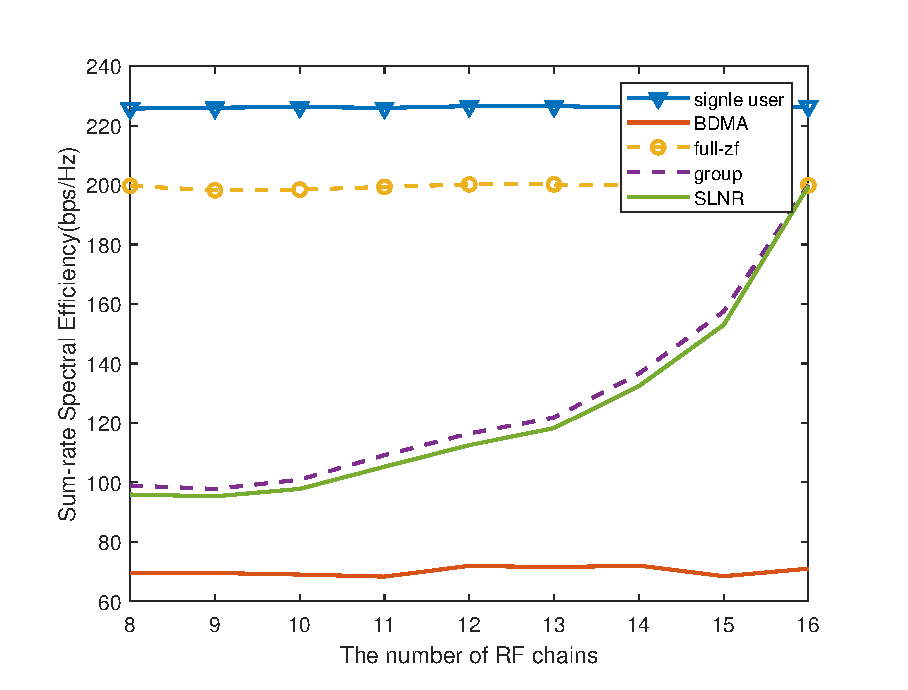
\includegraphics[width=3.8in,height=3.2in]{Figure/NRFChains.eps}
		\caption{Different number of RF chains.}\label{fig:RFchains}
	\end{center}
\end{figure}
In Fig.~\ref{fig:RFchains}, we can see that the sum-rate capacity will increase as more RF chains added. The upper bound is the zero-forcing precoding system with 16 RF chains for 16 users. The conventional ZF is the hybrid precoding system with 8 RF chains for 8 users.


\begin{figure}[ht]
	\begin{center}
		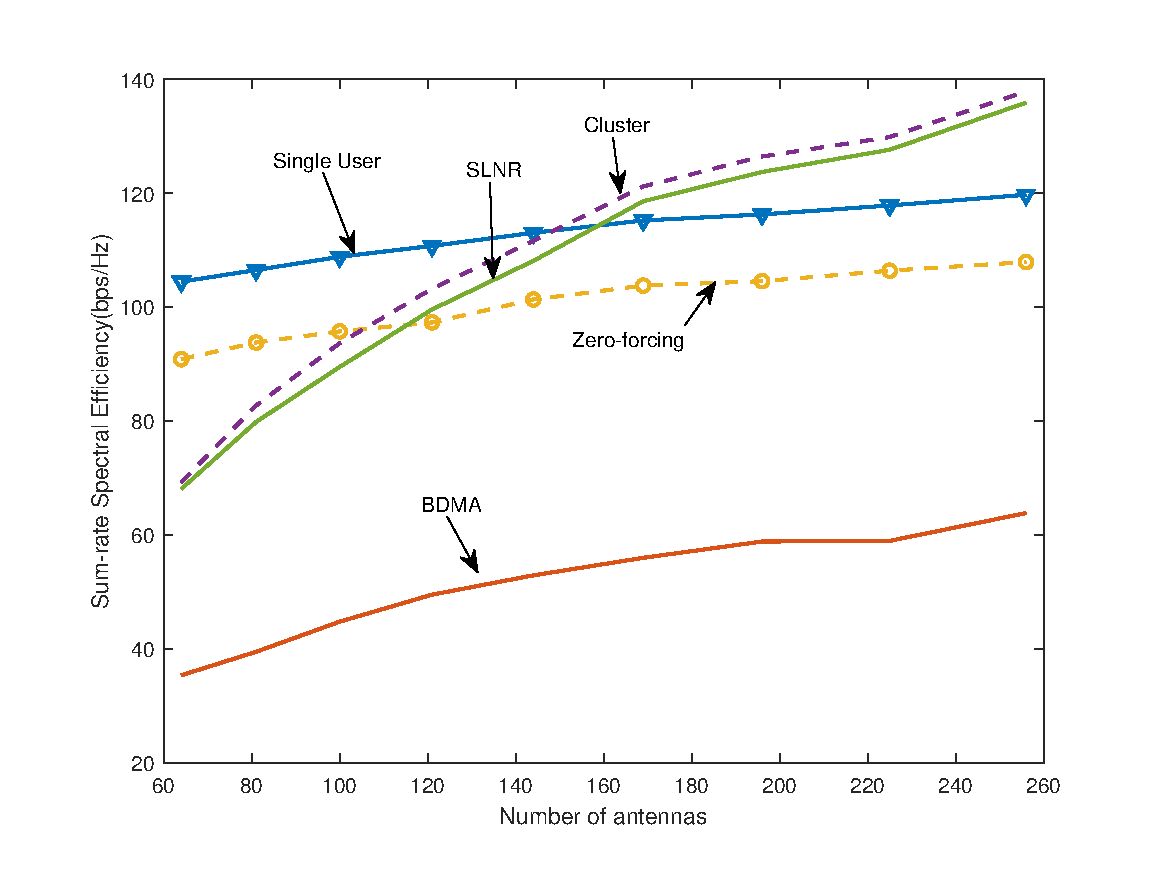
\includegraphics[width=3.8in,height=3in]{Figure/antenna.eps}
		\caption{The sum-rate capacity for different number of TX antennas.}\label{fig:CDF}
	\end{center}
\end{figure}

\begin{figure}[ht]
	\begin{center}
		\includegraphics[width=3.8in,height=3in]{Figure/differentcluster.eps}
		\caption{The sum-rate capacity for different number of TX antennas.}\label{fig:differentK}
	\end{center}
\end{figure}
The Fig. \ref{fig:differentK} shows that the BZF and BSM are lower bounded by the BDMA and upper bounded by conventional zero-forcing.

Finally, the performance for different systems with increasing number of antennas is shown in Fig. \ref{fig:CDF}. By varying the number of antennas, we investigate the sum-rate capacity improvement. The capacity of BZF and BSM will significantly increase as the more antennas. The reason is that the residual interference from Eq. \eqref{approx} will be reduced for more antennas.

\section{Conclusion}
In this work, we have developed block clustering precoding scheme for mmWave massive MIMO systems by jointly performing hybrid analog-digital precoding and user-beam clustering. First, we have modeled the block hybrid precoder design to reduce the required RF chains by processing the data streams cluster-by-cluster and the analog precoder can be solved by greedily maximizing the sum-SIR. Furthermore, two approaches are proposed, namely BZF and BSM, to obtain the digital precoder. Simulation results have confirmed that the proposed block clustering precoding scheme can achieve better sum-rate capacity with less RF chains compared to the conventional hybrid precoding scheme. The two approaches BZF and BSM can be considered to have the equivalent performance.


\bibliography{BDMAref}
\bibliographystyle{IEEEtran}


% references section

\end{document}


